\begin{figure}
	\centering
	\subfigure[Odziv na stopnico pri vzor\v{c}nem \v{c}asu 100 Hz]
	{
		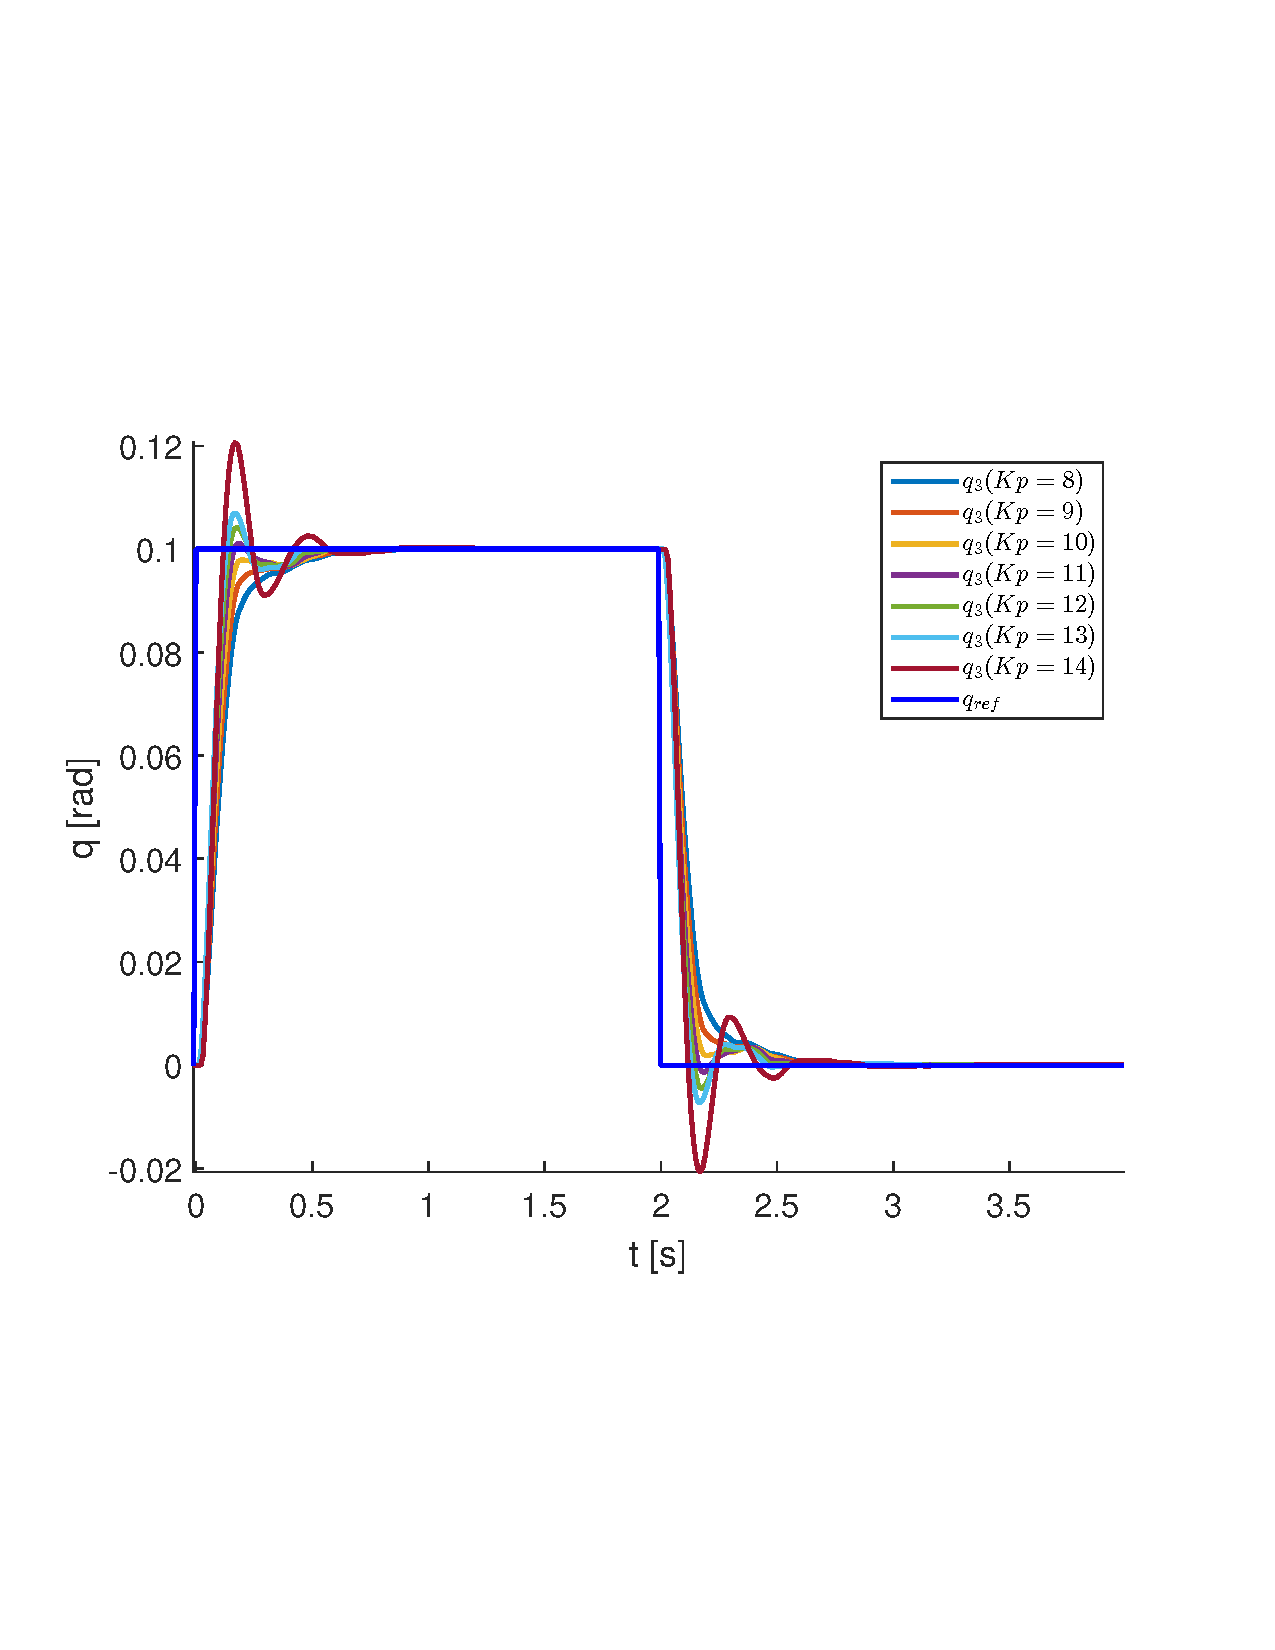
\includegraphics[trim={0 6cm 0 7cm},scale=0.5]{./Slike/follow_step_100hz_vel.pdf}
	}
	\subfigure[Odziv na stopnico pri vzor\v{c}nem \v{c}asu 500 Hz]
	{
		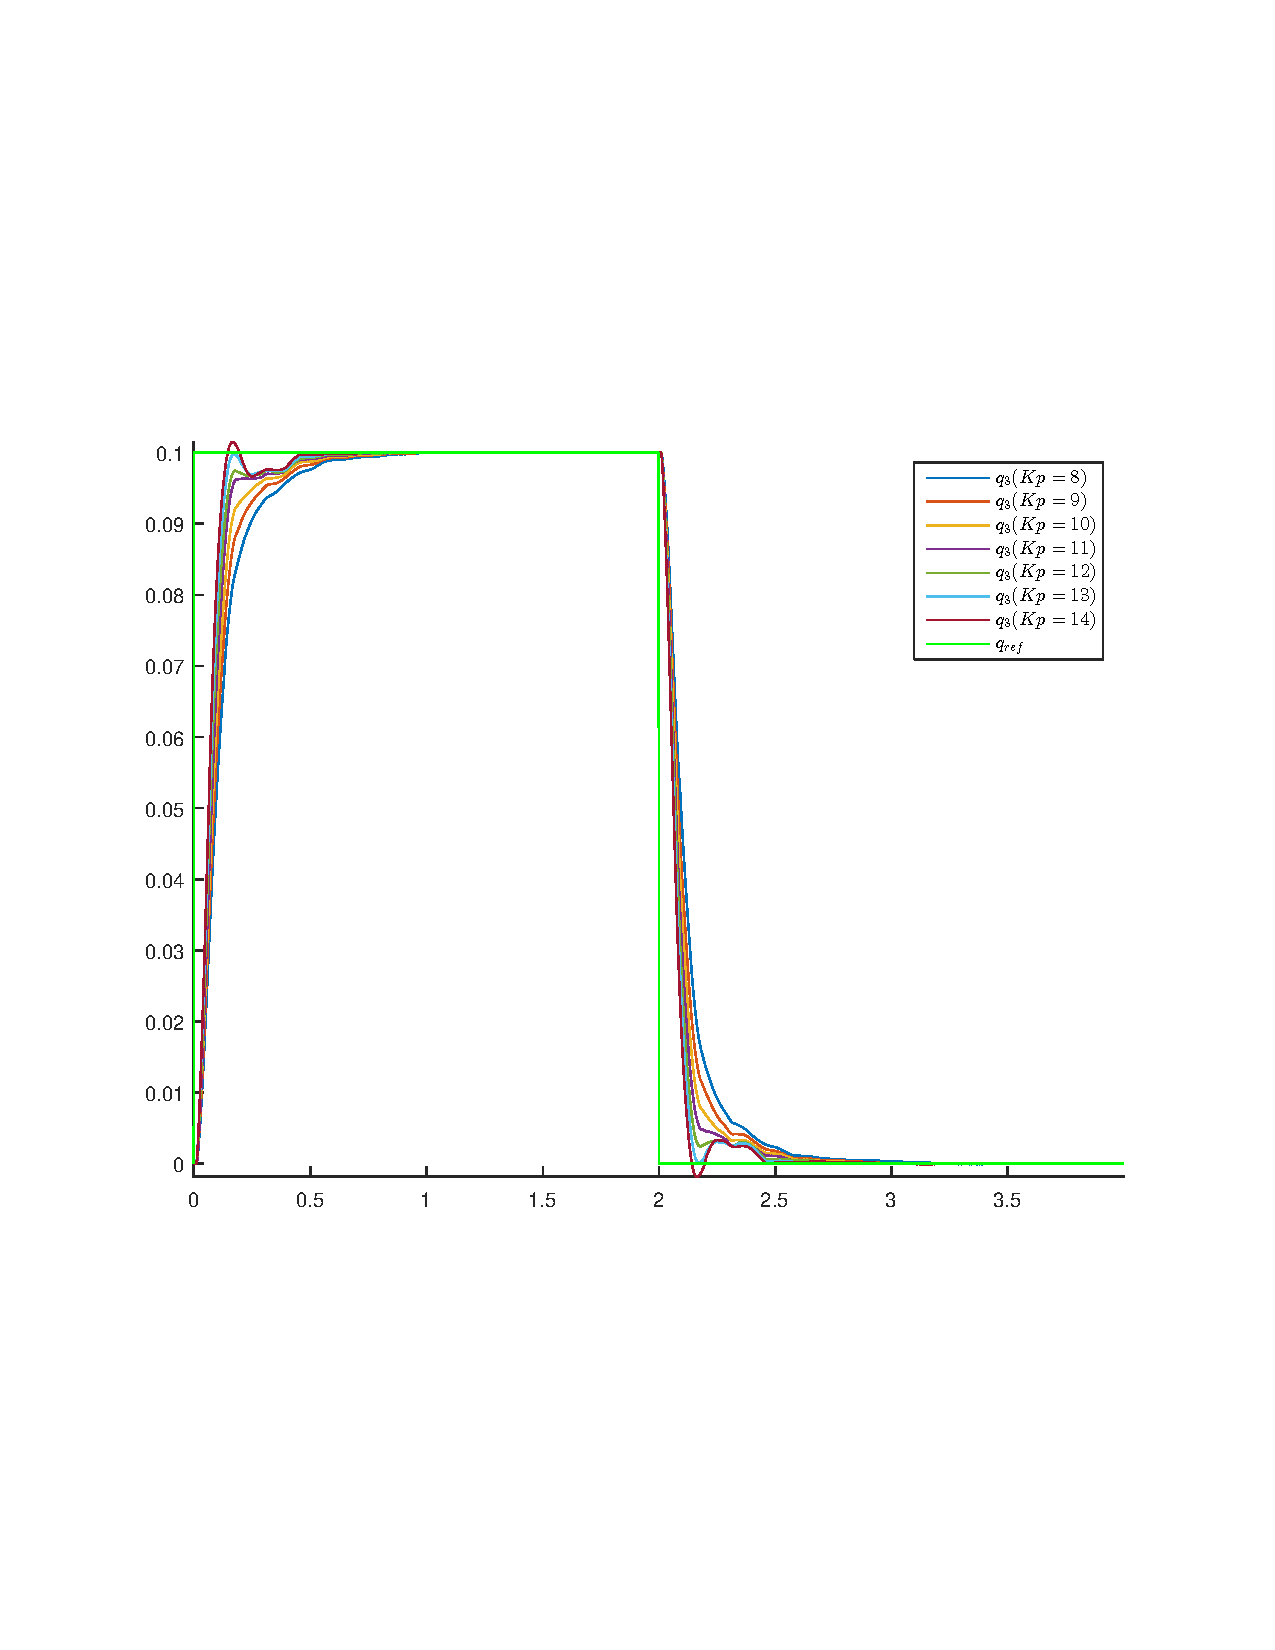
\includegraphics[trim={0 6cm 0 7cm},scale=0.5]{./Slike/follow_step_500hz_vel.pdf}
	}
	\caption{Odzivi tretjega sklepa na signal stopnice pri razli\v{c}nih oja\v{c}anjih in razli\v{c}nih vzor\v{c}nih \v{c}asu.}
	\label{fig:follow_step}
\end{figure}
